\documentclass[../../main.tex]{subfiles}

\usepackage{pgfplots}

\begin{document}

\chapter{Results}

A number of experiments were conducted with two broad goals: verifying that at least some of the proposed options work on simplified abstract engineering environments, and proving that the proposed architecture has desirable qualities in more complex environments.
Some experiments were also carried out to visualise and explore the latent space mappings in an intuitive way.

\section{Approach verification}

\subsection{Distribution distance}

Due to the potential issues with minimising KL-divergence discussed in \S 4.1.2, a highly simplified environment was devised in which the target distribution is known.
The target distribution was fixed as a standard normal distribution (constraints were not considered at this stage) and the generator's output distribution was modelled as a normal distribution whose mean and standard deviation were controllable parameters.

Although KL-divergence is analytically tractable for two normal distributions, it was estimated through sampling of the generated distribution as described in \S 4.1.1.
Trained variables were initialised such that the standard deviation started at $1$, while the initial mean was varied.

\begin{figure}
    \begin{center}
    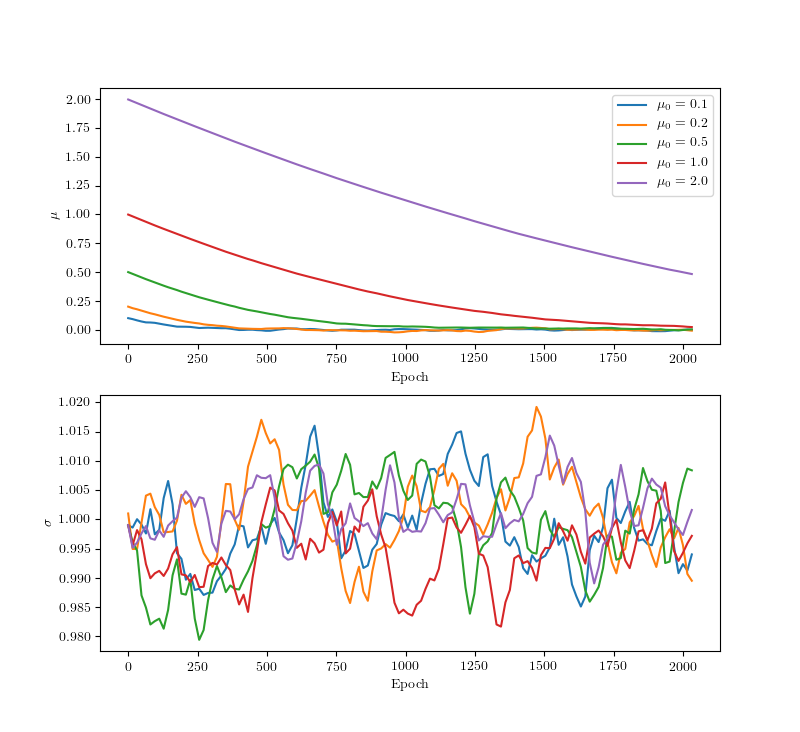
\includegraphics[width=\textwidth]{broadKLDivergence.png}
    \caption{
        Change in $\mu$ and $\sigma$ over time when training arbitrary normal distributions with different starting means to match the standard normal distribution. 
        Parameters were updated using the Adam optimisation algorithm to minimise KL-divergence, as estimated by taking samples from the varying distribution in batches of 64.
    }
    \label{fig:broadKLDivergence}
    \end{center}
\end{figure}

The mean $\mu$ and standard deviation $\sigma$ after each batch are shown in Figure \ref{fig:broadKLDivergence}.
Convergence does occur, but the time taken for the mean to approach $0$ appears to increase exponentially as the initial mean moves away from the target.
Two one-dimensional normal distributions whose means only differ by two and whose standard deviations are both one could still be considered to be quite close together, so the experiment was repeated with $\sigma=0.1$ for both distributions to better simulate disjoint distributions.

\begin{figure}
    \begin{center}
    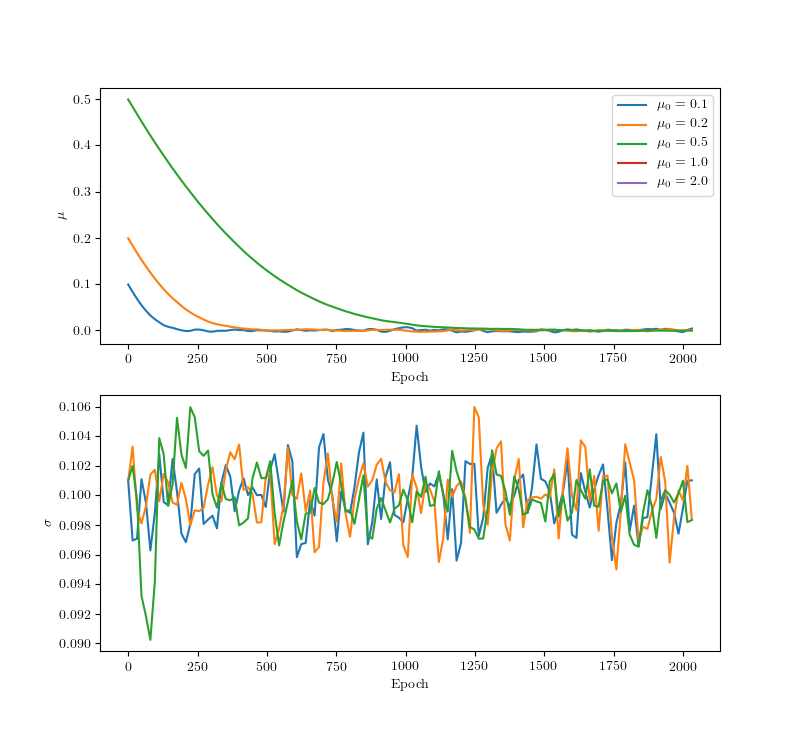
\includegraphics[width=\textwidth]{narrowKLDivergence.png}
    \caption{
        Change in $\mu$ and $\sigma$ over time when training arbitrary normal distributions with different starting means to match a normal distribution with $\mu=0$ and $\sigma=0.1$. 
        Parameters were updated using the Adam optimisation algorithm to minimise KL-divergence, as estimated by taking samples from the varying distribution in batches of 64.
    }
    \label{fig:narrowKLDivergence}
    \end{center}
\end{figure}

Figure \ref{fig:narrowKLDivergence} shows that the variables converge at approximately the same rate as when the standard deviation of the target distribution was $1$.
Missing, however, are the trend lines for $\mu_0=1.0$, $\mu_0=2.0$; both $\mu$ and $\sigma$ went to \url{NaN} after the first epoch.
This may well have been caused by an excessively large KL-divergence resulting in exploding gradients due to the limited precision of floating point numbers.

Changing the computation graph to use \url{float64} values instead of \url{float32} lends further evidence to this hypothesis, as increasing the precision allowed the $\mu=1.0, 2.0$, $\sigma=0.1$ cases to be optimised without numerical errors (Figure \ref{fig:narrowKLDivergenceFloat64}).
Similarly, using 16-bit floating point values always resulted in \url{NaN} errors occurring.

\begin{figure}
    \begin{center}
    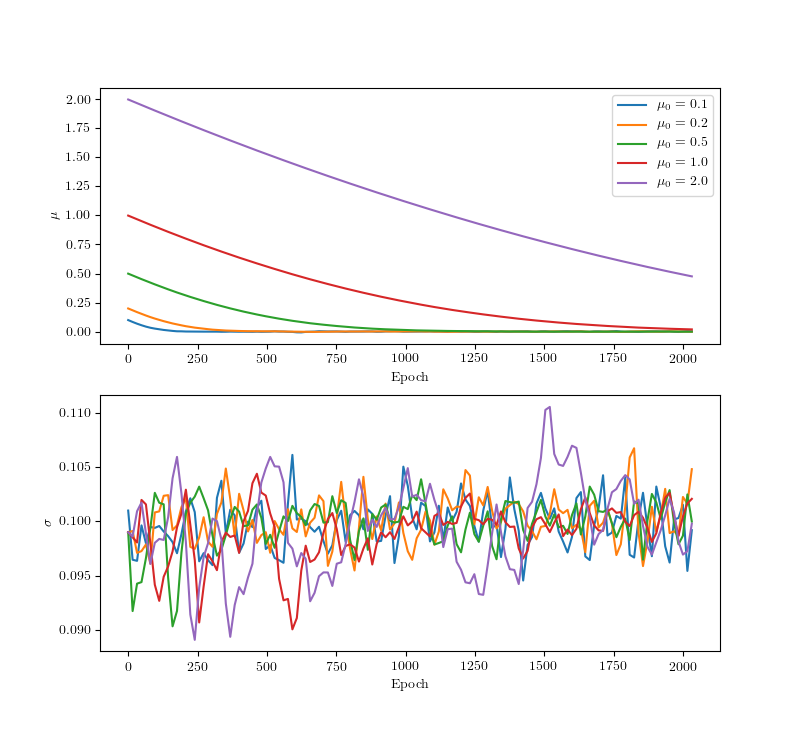
\includegraphics[width=\textwidth]{narrowKLDivergenceFloat64.png}
    \caption{
        Change in $\mu$ and $\sigma$ over time when training arbitrary normal distributions with different starting means to match a normal distribution with $\mu=0$ and $\sigma=0.1$. 
        Experimental parameters are the same as in Figure \ref{fig:narrowKLDivergence}, but with 64-bit floating point numbers as opposed to 32-bit.
    }
    \label{fig:narrowKLDivergenceFloat64}
    \end{center}
\end{figure}

It was therefore concluded that minimising KL-divergence is too inconsistent for practical use, as real distributions $-$ which are frequently disjoint $-$ would very likely cause numerical issues due to lack of the required precision.

\subsection{Precision proxy optimisation}

Potential issues with directly estimating the recall of one distribution with respect to another were discussed in \S 4.3.
It was also hypothesised that optimising only for precision, $\hat{p}(g)$, would result in the generator sampling only a small subset of the viable solutions.

A short experiment was devised to prove that this is the case and hence that some other approximation of the recall would be needed.
A function modelling the probability of satisfaction for a solution in one dimension ($m=1$) was defined arbitrarily as:
$$h(c,s) = \sigma(20c - 6) - \sigma(20c - 14)$$
where
$$\sigma(x)=\frac{1}{1+e^{-x}}$$
and there is only one possible constraint for the sake of simplicity ($n=0$).
A graph of the constraint satisfaction function on $[-1, 1]$ is shown in Figure \ref{fig:sigmoidBumpFunction}.
Numerically integrating $h$ between $c=-1$ and $c=1$ gives an area of $~0.3999$, so the probability density function is $\hat{V}(c)(s) \approx 2.5008 \; h(c,s)$.

\begin{figure}
    \begin{center}
    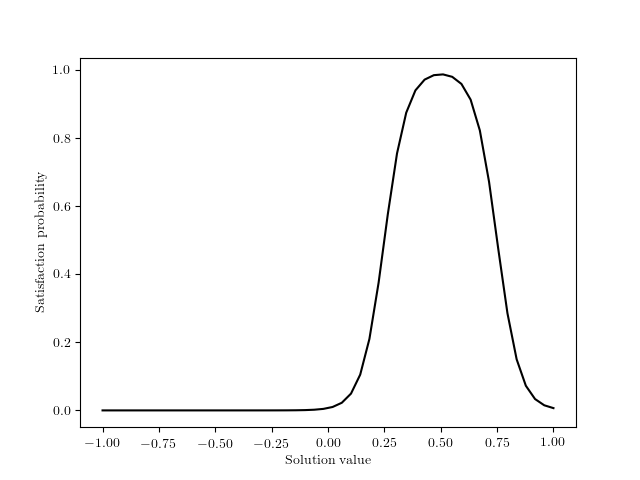
\includegraphics[width=\textwidth]{sigmoidBumpFunction.png}
    \caption{
        A test function estimating the probability that a solution $s$ satisfies a singular constraint $c$.
    }
    \label{fig:sigmoidBumpFunction}
    \end{center}
\end{figure}

Optimising the generator against $h(c, s)$ for the precision proxy defined in \S 4.2.1 consistently yields a distribution of generated solutions displayed in Figure \ref{fig:sigmoidBumpHistogram}.
Only considering precision and disregarding recall has clearly produced a mapping which is of no use: it always maps to the same point in spite of the fact that around $15\%$ of the solution space has a constraint satisfaction probability above $0.9$.

\begin{figure}
    \begin{center}
    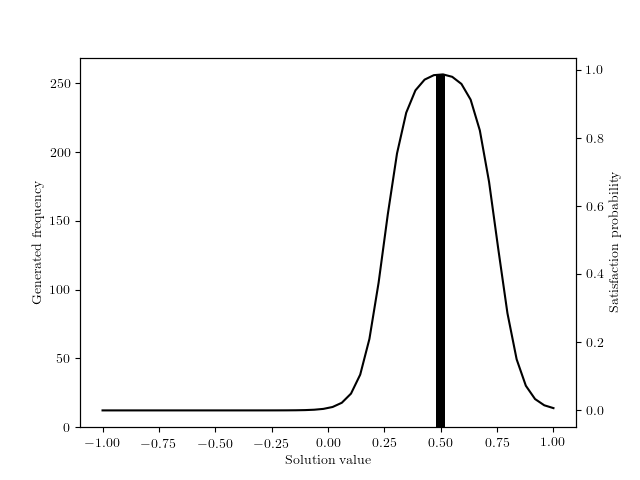
\includegraphics[width=\textwidth]{sigmoidBumpHistogram.png}
    \caption{
        Distribution of generated solutions compared to the constraint satisfaction function against which the generator was trained, in the form of a histogram consisting of 256 samples.
        The generator had two hidden layers, each with 8 leaky-ReLU activated units, and a single $\tanh$ output unit.
    }
    \label{fig:sigmoidBumpHistogram}
    \end{center}
\end{figure}

This issue becomes even more pronounced when the constraint satisfaction function is altered to have two distinct modes (Figure \ref{fig:sigmoidBumpHistogramBimodal}).
$$h(c,s) = \sigma(20c - 6) - \sigma(20c - 14) + \sigma(20c + 6) - \sigma(20c + 14)$$
While a very high precision is obtained, with all generated solutions having a satisfaction probability of $~96\%$, optimising solely for precision fails entirely to encapsulate the bimodality of the constraint satisfaction function even in such a simple environment, confirming that optimisation must take recall into consideration for satisfactory results.

\begin{figure}
    \begin{center}
    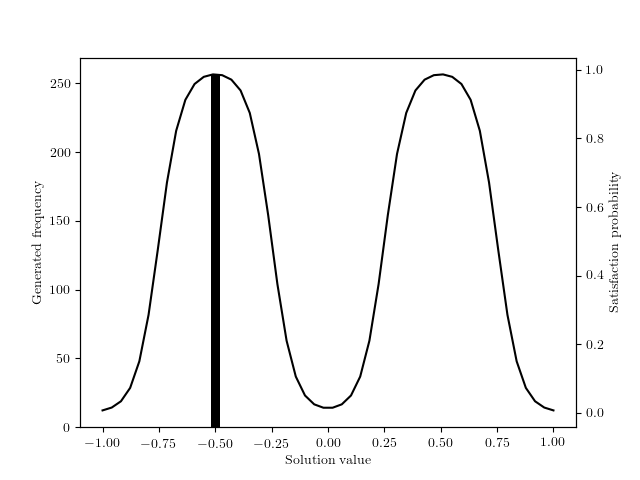
\includegraphics[width=\textwidth]{sigmoidBumpHistogramBimodal.png}
    \caption{
        Distribution of generated solutions compared to a bimodal constraint satisfaction function against which the generator was trained, in the form of a histogram consisting of 256 samples.
        The generator architecture is the same as that used in Figure \ref{fig:sigmoidBumpHistogram}.
    }
    \label{fig:sigmoidBumpHistogramBimodal}
    \end{center}
\end{figure}

\subsection{Pretraining}

In the absence of a recall proxy, it was suggested that the generator be pretrained to ensure that its initial distribution covers as wide a range of the solution space as possible.
This is based on two suppositions: that the generator initially only takes samples from an isolated region of the solution space; and that a more general distribution would explore multiple high-satisfaction regions of the solution space, thereby capturing a multimodal distribution even when optimising only for precision.
The generator's architecture remained the same as that used in \S 6.1.2, and the bimodal constraint satisfaction function from the latter half of that section was also used.

That the first assumption is true is confirmed trivially by taking samples from the generator before training (Figure \ref{fig:initialisedGenerator}).
Glorot initialisation, a common method of initialising the weights of neural networks, was used to initialise the generator's network weights.

\begin{figure}
    \centering
    \begin{subfigure}[a]{1.\textwidth}
        \centering
        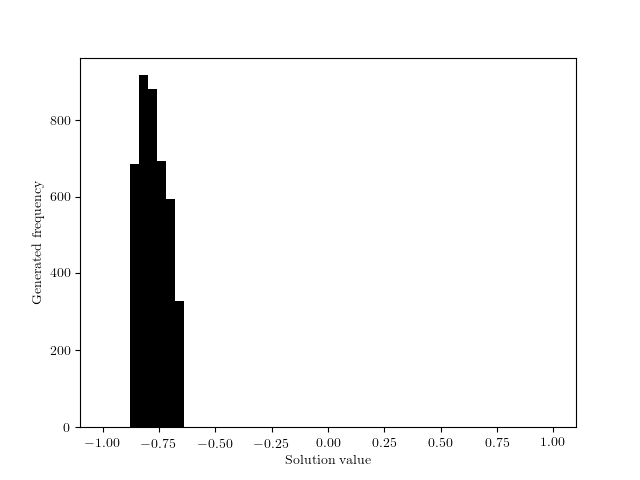
\includegraphics[width=0.6\textwidth]{initialisedGenerator1.png}
    \end{subfigure}
    \begin{subfigure}[a]{1.\textwidth}
        \centering
        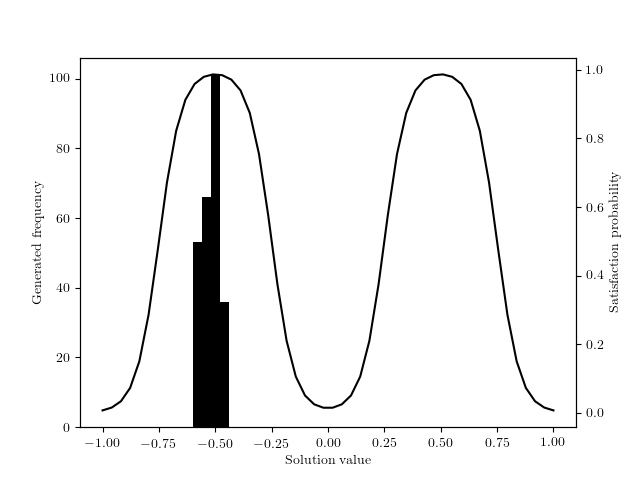
\includegraphics[width=0.6\textwidth]{initialisedGenerator2.png}
    \end{subfigure}
    \begin{subfigure}[a]{1.\textwidth}
        \centering
        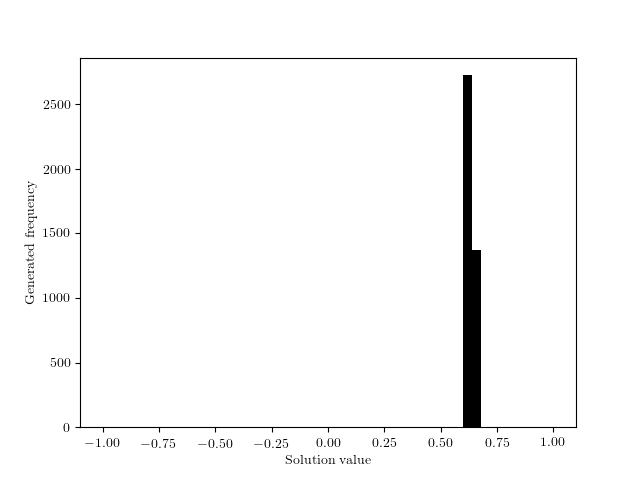
\includegraphics[width=0.6\textwidth]{initialisedGenerator3.png}
    \end{subfigure}
    \caption{
        Generated distribution immediately after network initialisation for three different seeds.
    }
\label{fig:initialisedGenerator}
\end{figure}

\subsection{Recall proxy optimisation}
\subsection{Constraint embeddings}

\section{Method properties}
\subsection{Expected satisfaction probability}
\subsection{Relative density of true solutions}
\subsection{Effect of recall weight}
\subsection{Multimodal solution sets}
\subsection{Equality constraints}

\section{Latent space properties}

\section{Application to complex problems}

\end{document}
